\documentclass[12pt,oneside]{article}

%%%%%%%%%%%%%%%%%%%%%%%%%%%%
%%   Zusaetzliche Pakete  %%
%%%%%%%%%%%%%%%%%%%%%%%%%%%%
\usepackage{enumerate}  
\usepackage{fancyhdr}
\usepackage{a4wide}
\usepackage{graphicx}
\usepackage{palatino}
\usepackage{multirow}
\usepackage{booktabs}
\usepackage{titlesec}
\usepackage{acronym}% http://ctan.org/pkg/acronym
\usepackage{enumitem}% http://ctan.org/pkg/enumitem

%folgende Zeile auskommentieren für englische Arbeiten
\usepackage[ngerman]{babel}
%folgende Zeile auskommentieren für deutsche Arbeiten
%\usepackage[ngerman, english]{babel}

\usepackage[T1]{fontenc}
\usepackage[utf8]{inputenc}
\usepackage[bookmarks]{hyperref}
\usepackage[justification=centering]{caption}
\usepackage[style=authoryear,natbib=true,backend=biber,maxbibnames=20]{biblatex}
\usepackage{csquotes}
\bibliography{literatur}

\setlength{\parindent}{0em} 
\setlist[itemize]{noitemsep, topsep=0pt}
\setlist[enumerate]{noitemsep, topsep=0pt}

\newcommand{\subsubsubsection}[1]{\paragraph{#1}\mbox{}\\}
\setcounter{secnumdepth}{4}
\setcounter{tocdepth}{4}
%%%%%%%%%%%%%%%%%%%%%%%%%%%%%%
%% Definition der Kopfzeile %%
%%%%%%%%%%%%%%%%%%%%%%%%%%%%%%

\pagestyle{fancy}
\fancyhf{}
\cfoot{\thepage}
\setlength{\headheight}{16pt}

%%%%%%%%%%%%%%%%%%%%%%%%%%%%%%%%%%%%%%%%%%%%%%%%%%%%%
%%  Deckblatt (Platzhalter)  %%
%%%%%%%%%%%%%%%%%%%%%%%%%%%%%%%%%%%%%%%%%%%%%%%%%%%%%
\thispagestyle{empty}
%Platzhalter für späteres Deckblatt
\hspace{-2cm}
\includegraphics{pabu5097_3677_cover.pdf}
\newpage

%%%%%%%%%%%%%%%%%%%%%%%%%%%%
%%  Beginn des Dokuments  %%
%%%%%%%%%%%%%%%%%%%%%%%%%%%%

\begin{document}

\lhead{}
\pagenumbering{Roman} 
    \setcounter{page}{1}

\tableofcontents
\clearpage

%%%%%%%%%%%%%%%%%%%%%%%%%%%%
%%  Kurzzusammenfassung   %%
%%%%%%%%%%%%%%%%%%%%%%%%%%%%
\lhead{Zusammenfassung}
%\section*{Zusammenfassung}
\addcontentsline{toc}{section}{Zusammenfassung}
\newpage
\newpage
\begin{otherlanguage}{ngerman}
\section*{Zusammenfassung}

In dieser Arbeit soll das Thema der forensischen Analyse von schädlicher Software behandelt werden. Explizit ist damit gemeint, dass eine Umgebung für diese Untersuchung in wenigen Sekunden geschaffen werden kann, welche den nötigen Sicherheitsstandards entspricht und so eine sichere Beobachtung des Malwareverhaltens gewährleisten kann. Diese Umgebung soll unabhängig vom Anbieter mit den selben Werkzeugen erstellt werden. So kann im Notfall schnell gehandelt werden, um festzustellen, welche Systemkomponenten von einem Angriff gefährdet sind.
\newline Somit ist diese Arbeit im Bereich der IT-Security und Datensicherheit anzusiedeln. Dies sind in der heutigen Zeit wichtige Themenbereiche um den Schutz aller Daten bieten zu können.
\end{otherlanguage}

\lhead{Abstract}
\section*{Abstract}
\addcontentsline{toc}{section}{Abstract}



\newpage
\lhead{Abbildungsverzeichnis} 
\addcontentsline{toc}{section}{Abbildungsverzeichnis} 
\listoffigures

\newpage
\lhead{Tabellenverzeichnis}
\addcontentsline{toc}{section}{Tabellenverzeichnis} 
\listoftables
\newpage

\setlength{\parskip}{0.5em} 


%%%%%%%%%%%%%%%%%%%%%%%%%%%%%%%%%%
%%  Definition der Abkürzungen  %%
%%%%%%%%%%%%%%%%%%%%%%%%%%%%%%%%%%
\lhead{Abkürzungsverzeichnis} 
\section*{Abkürzungsverzeichnis} 
\addcontentsline{toc}{section}{Abkürzungsverzeichnis}  

\begin{acronym}
 \acro{VM}{Virtuelle Maschine}
\end{acronym}
\newpage
%%%%%%%%%%%%%%%%%%%%%%%%%%%%
%%  Glossar  %%
%%%%%%%%%%%%%%%%%%%%%%%%%%%%
\lhead{Glossar} 
%\section*{Glossar} 
\addcontentsline{toc}{section}{Glossar}  
\newpage
\begin{otherlanguage}{ngerman}
\section*{Glossar}
\begin{acronym}
 \acro{App}{- ist eine Anwendung}
 \acro{Cloud}{- ist in der IT die Abkürzung für Cloud Computing und wird auch als Rechnerwolke oder Datenwolke bezeichnet}
 \acro{Cloud Server}{- ist ein virtueller Server. Dieser bezieht seine Hardwarekomponenten von externen Dienstleistern und wird über das Internet angeboten.}
 \acro{Firewall}{- ist ein Sicherungssystem um Netzwerke und Computer vor unerewünschten Zugriffen zu schützen}
 \acro{Open-Source-Software}{- ist Software deren Quellcode der Öffentlichkeit zugänglich ist. Die Benutzung des Codes steht dem Benutzer selbst offen.}
 \acro{OS-Images}{- ist eine komprimierte Sammlung von Referenzdateien und Ordnern, die zum Installieren und Konfigurieren eines neuen Betriebssystems auf einem Computer verwendet werden}
 \acro{Workflow}{- die Abwicklung arbeitsteiliger Vorgänge}
 \acro{Cloud Provider}{- Anbieter für Cloud Computing}
\end{acronym}
\end{otherlanguage}
%%%%%%%%%%%%%%%%%%%%%%%%%%%%
%%  Einstellungen  %%
%%%%%%%%%%%%%%%%%%%%%%%%%%%%
\clearpage
\pagenumbering{arabic}  
    \setcounter{page}{1}
\lhead{\nouppercase{\leftmark}}

%%%%%%%%%%%%%%%%%%%%%%%%%%%%
%%  Hauptteil  %%
%%%%%%%%%%%%%%%%%%%%%%%%%%%%
\lhead{Einleitung}
\section{Einleitung} 
-
\subsection{Fragestellung}
-am ende entscheiden ob der punkt drin bleibt oder nicht
\subsection{Forschungsstand}
-nennung von Messen wie bspw. defcon
\newline
-publikationen aus exposé-quellen einbeziehen
\subsection{Aufbau der Arbeit}
-von welchem Thema gehe ich zu welchem thema um roten faden darzulegen
\newpage

\lhead{Theoretische Grundlagen}
\section{Theoretische Grundlagen} 
%\subsection{Terraform}
\subsection{Terraform}
\begin{otherlanguage}{ngerman}
\subsubsection{Funktionsweise}
\textit{Terraform} ist eine \textit{Open-Source-Software}, welche die Vorbereitung von \textit{Cloud Servern} einfacher macht. Sie wurde von HashiCorp dazu entwickelt, Infrastrukturen vorzubereiten und zu verwalten.\footcite{introform} Mit Infrastrukturen sind hier \textit{virtuelle Maschinen} verschiedenster Anbieter gemeint.\footnote{\cite{Terraform}} Terraform hat lizenzierte Partner für die seine Dienste anwendbar sind.\footcite{TerraProviders} Durch die hohe Konnektivität dieser Software sind die Einsatzorte sehr vielseitig. Das macht die Software in der Entwicklung und im Betrieb von Unternehmen sehr attraktiv. 
\newline
\newline
Terraform ist ein Infrastructure-as-Code-Tool und wird für die Bereitstellung von physischen als auch virtuellen Servern verwendet. Das Tool arbeitet mit Konfigurationsdateien, die in der HashiCorp Configuration Language(HCL) geschrieben werden. Die genannten Dateien sind von Menschen lesbar und gewährleisten dadurch die geringe Komplexität der Sprache. Zudem ist HCL eine deklarative Sprache. Das heißt, dass der Nutzer den Wunschaufbau des Servers in der Terraform-Datei beschreibt. Die einzelnen Schritte um den gewünschten Serverzustand zu erreichen werden von Terraform übernommen. 
\newline
Die Prozesse in die die Arbeit mit Terraform unterschieden werden kann, sind in drei Schritte aufgeteilt. Der erste Schritt ist \tt write \rm. In dieser Phase wird der Code definiert. Dafür werden die benötigten Ressourcen für die jeweiligen Provider definiert. Dafür Terraform-Konfigurations-Dateien mit der Endung \tt .tf \rm verwendet. Aus diesen Dateien entnimmt Terraform beispielsweise welcher Cloud-Anbieter verwendet wird. Als Beispiel für einen Anbieter mit dem Terraform funktioniert können die Microsoft Azure-Dienste genannt werden. Zu den Providern findet sich auf der Seite von Terraform eine jeweilige Dokumentation darüber, wie die Ressourcen einzubinden sind. Der Code der Konfigurations-Dateien entscheidet darüber, wie der Server konfiguriert wird, wenn dass script ausgeführt wird. 
\newline
Wenn der Code verfasst wurde folgt der nächste Schritt im Arbeitsablauf von Terraform. Dieser ist die Planung der vorgenommenen Aktionen. Wird \tt terraform apply \rm in der Kommandozeile eingegeben so wird dieser Plan erstellt. Dieser wird im Anschluss daran ausgegeben. Um Fortzufahren muss der Plan, indem jeder Schritt aufgelistet ist, den Terraform durchführen wird, bestätigt werden. Diese einzelnen Schritte können Änderungen, Löschungen oder das Hinzufügen von Dateien sein.
\begin{figure}
    \centering
    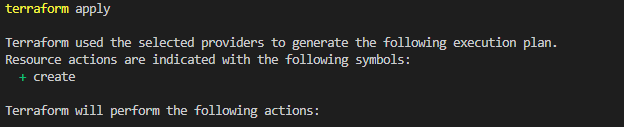
\includegraphics{LaTeX/graphic/terraformapply.png}
    \caption{Terraform - Planungsphase}
\end{figure}
%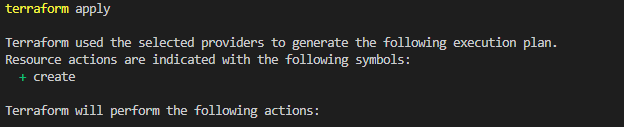
\includegraphics[]{LaTeX/graphic/terraformapply.png}

\newpage 
Die Dritte und letzte Phase im Terraform-Workflow ist \tt apply \rm. Sie beginnt mit der Bestätigung des Plans. Ab diesem Zeitpunkt beginnt Terraform mit der Bereitstellung des Servers. Welche Systemkomponenten und Sicherheitseinstellungen dieser hat ist von den Konfigurationsdateien abhängig. 
\newpage
\subsubsection{Vorteile}
-schnell
\newline
-variabel
\newline
-nicht allzu komplex
\end{otherlanguage}

\subsection{Virtuelle Maschinen}
\subsubsection{Was ist eine virtuelle Maschine?}
-Anwendungsumgebung
\newline
-Hardware imitiert

\subsubsection{Erstellen einer virtuellen Maschine}
-terraform einbringen und allgemeines vorgehen beschreiben wie es ohne terraform wäre
\newline
-überleitung absicherung
\subsubsection{Absicherung einer virtuellen Maschine}
-firewall 
\newline
-was für absicherungen sollten getroffen werden
\newline
-firewall konfiguration erklären
\subsection{Malware}
\subsubsection{Was ist Malware?}
-Schadcode 
\newline
-wurde dazu entwickelt schaden anzurichten
\newline
-nicht politisch werden!!! (nicht gru mit einbeziehen)
\subsubsection{Arten von Malware}
-virus
\newline
-Würmer
\newline
-trojaner
\newline
-Spyware
\newline
-Scareware
\newline
-Ransomware
\newline
-alle kurz anschneiden aber nicht zu tief
\subsection{Malware-Analyse}
- in den unteren 4 Punkten die Malwareanalyse erklären und auch den forschungsstand mit einbeziehen
\subsubsection{Einfache statische Analyse}
\subsubsection{Einfache dynamische Analyse}
\subsubsection{Erweiterte statische Analyse}
\subsubsection{Erweiterte dynamische Analyse}
\newpage

\lhead{Methodik}
\section{Methodik}
\subsection{Terraform}
- configs zeigen und einzelne befehle erklären: warum mache ich was
\subsection{Virtuelle Umgebung}
-was habe ich wo und wie gemacht
\newline
-mit screenshots dokumentieren und untermauern an passenden stellen
\subsection{Tools}
- UNBEDINGT RANSETZEN
\subsection{Malware}
- kurze Erklärung, dass ich Malware hab
\newpage

\lhead{Ergebnisse}
\section{Ergebnisse}
\newpage

\lhead{Bewertung der Ergebnisse}
\section{Bewertung des Ergebnisses}
\subsection{Vorteile der Vorgehensweise}
\subsection{Nachteile der Vorgehensweise}
\newpage

\lhead{Diskurs}
\section{Diskurs}
\subsection{Schlussbetrachtung}
\subsection{Ausblick}
\newpage 


\lhead{Literatur- und Quellenverzeichnis}
\section{Literatur- und Quellenverzeichnis}
%%%%%%%%%%%%%%%%%%%%%%%%%%%%
%% Literaturverzeichnis wird 
%% automatisch eingefügt
%%%%%%%%%%%%%%%%%%%%%%%%%%%%

\printbibliography
\addcontentsline{toc}{section}{Literatur- und Quellenverzeichnis}
aufteilen in internetquellen
publications
books

\newpage
\lhead{Anhang}
\section{Anhang}
\appendix
\section{Anhang A} 





%%%%%%%%%%%%%%%%%%%%%%%%%%%%
%% Eidesstattliche Erklärung
%%%%%%%%%%%%%%%%%%%%%%%%%%%%
\clearpage
\newpage
\begin{otherlanguage}{ngerman}
\thispagestyle{empty}
\section*{Eidesstattliche Erklärung}
\thispagestyle{empty}
Hiermit versichere ich, die vorliegende Arbeit selbstständig verfasst und keine anderen als die angegebenen Quellen und Hilfsmittel benutzt sowie die Zitate deutlich kenntlich gemacht zu haben.
\newline
Ich erkläre weiterhin, dass die vorliegende Arbeit in gleicher oder ähnlicher Form noch nicht im Rahmen eines
anderen Prüfungsverfahrens eingereicht wurde.
\vspace{4\baselineskip}\\
Berlin, den \today \hfill Patrick Lucas Büdke 
\vspace{4\baselineskip}\\
\end{otherlanguage}

\end{document}
